
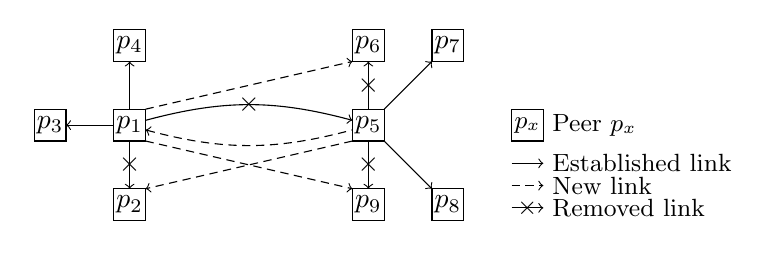
\begin{tikzpicture}[scale=1.15]
  
  \draw[fill=white] (0pt, 0pt) node{$p_1$} +(-5pt,-5pt) rectangle +(5pt,5pt);
  \draw[fill=white] ( 0pt,-25pt) node{$p_2$} +(-5pt,-5pt) rectangle +(5pt,5pt);
  \draw[fill=white] (-25pt,0pt) node{$p_3$} +(-5pt,-5pt) rectangle +(5pt,5pt);
  \draw[fill=white] ( 0pt,25pt) node{$p_4$} +(-5pt,-5pt) rectangle +(5pt,5pt);

  \draw[->] (-5pt, 0pt) -- (-20pt, 0pt); %% p1 -> p2
  \draw[->] ( 0pt, 5pt) -- (  0pt,20pt); %% p1 -> p3
  \draw[->] ( 0pt,-5pt) -- node{$\times$} (  0pt,-20pt); %% p1 -> p4
  
  \begin{scope}[shift={(75pt,0pt)}]
  \draw[fill=white] ( 0pt, 0pt) node{$p_5$} +(-5pt,-5pt) rectangle +(5pt,5pt);
  \draw[fill=white] (0pt,  25pt) node{$p_6$} +(-5pt,-5pt) rectangle +(5pt,5pt);
  \draw[fill=white] ( 25pt,25pt) node{$p_7$} +(-5pt,-5pt) rectangle +(5pt,5pt);
  \draw[fill=white] (25pt,-25pt) node{$p_8$} +(-5pt,-5pt) rectangle +(5pt,5pt);
  \draw[fill=white] (0pt, -25pt) node{$p_9$} +(-5pt,-5pt) rectangle +(5pt,5pt);

  \draw[->] ( 5pt, 5pt) -- ( 20pt, 20pt);
  \draw[->] ( 5pt, -5pt) -- ( 20pt,-20pt);
  \draw[->] ( 0pt, 5pt) -- node{$\times$} ( 0pt,20pt);
  \draw[->] ( 0pt,-5pt) -- node{$\times$} ( 0pt,-20pt);
  \end{scope}
  
  \draw[->, densely dashed] (5pt,5pt) -- (70pt,20pt); 
  \draw[->, densely dashed] (70pt,-5pt) -- (5pt,-20pt);
  \draw[->, densely dashed] ( 5pt,-5pt) -- (70pt,-20pt);
  \draw[->] (5pt, 1.5pt) to[out=15,in=165]
  node{$\times$} (70pt, 1.5pt);
  \draw[<-, densely dashed] (5pt, -1.5pt) to[out=-15,in=-165] (70pt,-1.5pt);

  \small 
  \begin{scope}[shift={(120pt,0pt)}]
    \draw[fill=white](5pt, 0pt)node{$p_x$}+(-5pt,-5pt) rectangle +(5pt,5pt);
    \draw (10pt,0pt) node[anchor=west]{Peer $p_x$};
    \draw[->](0pt, -12pt)--(10pt, -12pt) node[anchor=west]{Established link};
    \draw[->, densely dashed](0pt, -19pt)--(10pt, -19pt)
    node[anchor=west]{New link};
    \draw[->](0pt, -26pt)-- node{$\times$}(10pt, -26pt)
    node[anchor=west]{Removed link};
    
  \end{scope}
  
\end{tikzpicture}